\documentclass[output=paper,colorlinks,citecolor=brown,
% hidelinks,
% showindex
]{langscibook}
\author{Hagen Pitsch\affiliation{University of Göttingen}\orcid{0000-0002-7575-8903}}
\title{Slovak verbal inflection in a declarative lexicalist approach to morphology}
\abstract{Inspired by \citet{Zimmermann2019} who ventured on the task to model Spanish verbal inflection within a declarative approach to morphology, the present contribution seeks to do something similar with respect to Slovak. The paper provides readers with basic facts about Slovak phonology and verbal paradigms, outlines the essentials of the framework, and tries to reconstruct how (first and second-language) learners of Slovak are likely to deduce word-schemas (generalizations) on the basis of the input they are exposed to. Ultimately, a moderate word-form lexicon is suggested to be the most cognitively realistic scenario of lexical access.}
  
%move the following commands to the "local..." files of the master project when integrating this chapter
\usepackage{tabularx}
\usepackage{langsci-basic}
\usepackage{langsci-optional}
\usepackage{langsci-gb4e}
\bibliography{localbibliography}
\newcommand{\orcid}[1]{}
\pagenumbering{roman}
\usepackage{tabto}
\usepackage{tipa}
\usepackage{stmaryrd}
\usepackage[linguistics]{forest}
\usepackage{multirow}
\usepackage{textgreek}
\usepackage{tikz}
\usetikzlibrary{arrows, fit, positioning, shapes}

\IfFileExists{../localcommands.tex}{%hack to check whether this is being compiled as part of a collection or standalone
   \usepackage{langsci-optional}
\usepackage{langsci-gb4e}
\usepackage{langsci-lgr}

\usepackage{listings}
\lstset{basicstyle=\ttfamily,tabsize=2,breaklines=true}

%added by author
% \usepackage{tipa}
\usepackage{multirow}
\graphicspath{{figures/}}
\usepackage{langsci-branding}

   
\newcommand{\sent}{\enumsentence}
\newcommand{\sents}{\eenumsentence}
\let\citeasnoun\citet

\renewcommand{\lsCoverTitleFont}[1]{\sffamily\addfontfeatures{Scale=MatchUppercase}\fontsize{44pt}{16mm}\selectfont #1}
  
   %% hyphenation points for line breaks
%% Normally, automatic hyphenation in LaTeX is very good
%% If a word is mis-hyphenated, add it to this file
%%
%% add information to TeX file before \begin{document} with:
%% %% hyphenation points for line breaks
%% Normally, automatic hyphenation in LaTeX is very good
%% If a word is mis-hyphenated, add it to this file
%%
%% add information to TeX file before \begin{document} with:
%% %% hyphenation points for line breaks
%% Normally, automatic hyphenation in LaTeX is very good
%% If a word is mis-hyphenated, add it to this file
%%
%% add information to TeX file before \begin{document} with:
%% \include{localhyphenation}
\hyphenation{
affri-ca-te
affri-ca-tes
an-no-tated
com-ple-ments
com-po-si-tio-na-li-ty
non-com-po-si-tio-na-li-ty
Gon-zá-lez
out-side
Ri-chárd
se-man-tics
STREU-SLE
Tie-de-mann
}
\hyphenation{
affri-ca-te
affri-ca-tes
an-no-tated
com-ple-ments
com-po-si-tio-na-li-ty
non-com-po-si-tio-na-li-ty
Gon-zá-lez
out-side
Ri-chárd
se-man-tics
STREU-SLE
Tie-de-mann
}
\hyphenation{
affri-ca-te
affri-ca-tes
an-no-tated
com-ple-ments
com-po-si-tio-na-li-ty
non-com-po-si-tio-na-li-ty
Gon-zá-lez
out-side
Ri-chárd
se-man-tics
STREU-SLE
Tie-de-mann
}
    \bibliography{localbibliography}
    \togglepaper[23]
}{}

\begin{document}
\shorttitlerunninghead{Slovak verbal inflection}
\maketitle

% %%%%%%%%%%%%%%%%%%%%%%%%%%%%%%%%%%%%%%%%%%%%%%%%%%%%%%%%%%%%%%%
% %%%%%%%%%%%%%%%%%%%%%%%%%%%%%%%%%%%%%%%%%%%%%%%%%%%%%%%%%%%%%%%

\section{Introduction}\label{sec:Intro}

In one of her last papers, Ilse \citet{Zimmermann2019} pursued a new avenue in her research agenda: She explored the theoretical possibility of a declarative (word-based) rather than a derivational (morpheme-based) approach to verb forms, and she demonstrated its possibilities for Spanish. As she states in a footnote, the appeal of such an approach was partially also based on her personal experience as a foreign language teacher. More generally, she felt the urgency of the question of what constitutes the difference between the two approaches with regard to the phenomena of linguistic competence and language acquisition.\footnote{``In meinen bisherigen Arbeiten zur Laut-Bedeutungszuordnung bin ich immer einer lexikali\-stischen Position gefolgt. Eine deklarative Betrachtungsweise probiere ich erstmals in der vorliegenden Studie aus. Angesichts meiner Erfahrungen als Fremdsprachenlehrkraft erscheint sie mir verlockend. Ganz allgemein stellt sich ja die Frage, was für die Phänomene der Sprachkompetenz und des Spracherwerbs der Unterschied zwischen derivationellen vs. deklarativen Aspekten in den verschiedenen Grammatikmodellen ausmacht.'' \citep[1]{Zimmermann2019} [``So far in all of my work on sound–meaning correspondence I have adhered to a lexicalist position. In the present study, I try to pursue a declarative approach for the first time. Due to my experience as a foreign-language teacher [in the far past; added by the editors], this approach seems to me appealing. In general, the question arises what consequences the differences between derivational vs. declarative aspects have for the treatment of the phenomena of language competence and language acquisition in the different models of grammar.'' (translation mine)]}

The present contribution seeks to explore the same path, but with regard to Slovak, a West Slavic language. I would like to show that the declarative way of treating Slovak verbs -- and Slavic in general -- is indeed promising and has a number of advantages as compared to (purely) derivational approaches. 

The paper is structured as follows: As a basis, \sectref{sec:SlovakPhonology} and \sectref{sec:SlovakVerbs} provide necessary pieces of information on Slovak phonology and verbal paradigms, respectively. \sectref{sec:Schemas} introduces the crucial concept of word-schemas, while \sectref{sec:LexEntries} is concerned with the format of lexical entries. \sectref{sec:Decomposing} is dedicated to reconstructing the process of creating word-schemas by learners of Slovak, tackling major verbal inflectional categories. \sectref{sec:Summary} summarizes the paper.

% %%%%%%%%%%%%%%%%%%%%%%%%%%%%%%%%%%%%%%%%%%%%%%%%%%%%%%%%%%%%%%%
% %%%%%%%%%%%%%%%%%%%%%%%%%%%%%%%%%%%%%%%%%%%%%%%%%%%%%%%%%%%%%%%

\section{Some notes on Slovak phonology}\label{sec:SlovakPhonology}

Codified standard Slovak has the six short vowel phonemes in \REF{ex:ShortVowels} (see \citealt[534]{Short1993}; orthographic representations added in angle brackets).

\ea\label{ex:ShortVowels}
\ea front vowels: /\ae/ $\langle$ä$\rangle$ -- /e/ $\langle$e$\rangle$ -- /i/ $\langle$i/y$\rangle$ 
\ex back vowels: /a/ $\langle$a$\rangle$ -- /o/ $\langle$o$\rangle$ -- /u/ $\langle$u$\rangle$
\z\z

\noindent However, only about 5\% of Slovak speakers are observed to pronounce /\ae/, while most speakers merge it with /e/ (see, a.o., \citealt[534]{Short1993}; \citealt[375]{Hanulikova.Hamann2010}).

The system of long vowel phonemes (i.e., vowels in long syllables) is more complex: Here we find the five phonemes in \REF{ex:LongVowels} as well as the four diphthongs in \REF{ex:Diphthongs} \citep[see][534]{Short1993}.\footnote{There is no diphthong corresponding to /iː/.}

\ea
\ea /aː/ $\langle$á$\rangle$ -- /eː/ $\langle$é$\rangle$ -- /iː/ $\langle$í,ý$\rangle$ -- /oː/ $\langle$ó$\rangle$ -- /uː/ $\langle$ú$\rangle$ \label{ex:LongVowels}
\ex /ia/ $\langle$ia$\rangle$ -- /ie/ $\langle$ie$\rangle$ -- /uo/ $\langle$ô$\rangle$ -- /iu/ $\langle$iu$\rangle$ \label{ex:Diphthongs}
\z\z

\noindent The long vowels in \REF{ex:LongVowels} are supplemented by the diphthongs in \REF{ex:Diphthongs} in the following way: While the latter occur only after palatal(ized) consonants, the former never do.\footnote{Slovak has only four truly palatal consonants, namely /d'/, /t'/, /n'/, and /l'/. Other ``soft'' consonants result from palatalization that occurs when the consonant precedes either of the front vowels /e/ and /i/. Moreover, some consonants are ``historically soft'', e.g. the affricate /c/ in \textit{vraciam} `(I) return'. In what follows, I note palatalization of underlyingly ``hard'' consonants only where it cannot be inferred from their position before a front vowel.} So both sets are in complementary distribution, while together they are in opposition to the matching short vowels in \REF{ex:ShortVowels}. This system of oppositions is depicted in \tabref{tab:pitsch:5}.\footnote{/C/ and /C'/ stand for any non-palatal or palatal consonant, respectively. Note that /aː/ may occur after the palatal /j/ under certain morphological conditions, and that /eː/ and /oː/ occur in borrowings only. /o:/ and /uo/ are not subject to the non-/palatal restriction and are therefore not in the table. /iu/ is restricted to few morphologically restricted environments.}

% % % % % % % % % % % % % % %
% TABELLE 5 VOWELS

\begin{table}
\caption{Vowel oppositions}
\label{tab:pitsch:5}
 \begin{tabular}{cccc}
  \lsptoprule
  \multirow{2}{*}{short} & & \multicolumn{2}{c}{long} \\
  & & after /C/ & after /C'/ \\
  \midrule
  /a/ $\langle$a$\rangle$ & : & /aː/ $\langle$á$\rangle$ & /ia/ $\langle$ia$\rangle$ \\
  /e/ $\langle$e$\rangle$ & : & /eː/ $\langle$é$\rangle$ & /ie/ $\langle$ie$\rangle$ \\
  /i/ $\langle$i/y$\rangle$ & : & \multicolumn{2}{c}{/iː/ $\langle$í/ý$\rangle$} \\
  /u/ $\langle$u$\rangle$ & : & /uː/ $\langle$ú$\rangle$ & /iu/ $\langle$iu$\rangle$ \\
  \lspbottomrule
 \end{tabular}
\end{table}

Most relevant in the context of Slovak verbal paradigms will be the phonemes  /a/--/aː/--/ia/, /e/--/eː/--/ie/, and /i/--/iː/.

% %%%%%%%%%%%%%%%%%%%%%%%%%%%%%%%%%%%%%%%%%%%%%%%%%%%%%%%%%%%%%%%
% %%%%%%%%%%%%%%%%%%%%%%%%%%%%%%%%%%%%%%%%%%%%%%%%%%%%%%%%%%%%%%%

\section{Slovak verbal paradigms}\label{sec:SlovakVerbs}

Slovak has only two synthetic finite verb forms: the present tense (see Tables \ref{tab:pitsch:1} and \ref{tab:pitsch:2}) and the imperative mood (\tabref{tab:pitsch:3}). Of non-finite forms, it features an infinitive, three participles, and the so-called transgressive (gerund); see \tabref{tab:pitsch:4}.\footnote{I omit the gerund in \tabref{tab:pitsch:4} since it can be easily derived by removing the agreement marker from active participles (e.g., \textit{volajúc-a} $\rightarrow$ `calling-\textsc{sg.f}' \textit{volajúc} `calling').}

% % % % % % % % % % % % % % % 
% TABELLE 1 PRÄSENS

\begin{table}[H]
\caption{Present-tense paradigms 1/2}
\label{tab:pitsch:1}
 \begin{tabular}{llllll}
  \lsptoprule
            & `call' & `return' & `understand' & `do' & `see' \\
  \midrule
  \textsc{1sg} & volám & vraciam & rozumiem & robím & vidím \\
  \textsc{2sg} & voláš & vraciaš & rozumieš & robíš & vidíš \\
  \textsc{3sg} & volá & vracia & rozumie & robí & vidí \\
  \textsc{1pl} & voláme & vraciame & rozumieme & robíme & vidíme \\
  \textsc{2pl} & voláte & vraciate & rozumiete & robíte & vidíte \\
  \textsc{3pl} & volajú & vracajú & rozumejú & robia & vidia \\
  \lspbottomrule
 \end{tabular}
\end{table}

% % % % % % % % % % % % % % %
% TABELLE 2 PRÄSENS

\begin{table}
\caption{Present-tense paradigms 2/2}
\label{tab:pitsch:2}
 \begin{tabular}{llllll}
  \lsptoprule
            & `hide' & `buy' & `forget' & `postpone' & `carry' \\
  \midrule
  \textsc{1sg} & skryjem & kupujem & zabudnem & odsuniem & nesiem \\
  \textsc{2sg} & skryješ & kupuješ & zabudneš & odsunieš & nesieš \\
  \textsc{3sg} & skryje & kupuje & zabudne & odsunie & nesie \\
  \textsc{1pl} & skryjeme & kupujeme & zabudneme & odsunieme & nesieme \\
  \textsc{2pl} & skryjete & kupujete & zabudnete & odsuniete & nesiete \\
  \textsc{3pl} & skryjú & kupujú & zabudnú & odsunú & nesú \\
  \lspbottomrule
 \end{tabular}
\end{table}

% % % % % % % % % % % % % % %
% TABELLE 3 IMPERATIV

\begin{table}
\caption{Imperative forms}
\label{tab:pitsch:3}
 \begin{tabular}{llll}
  \lsptoprule
  & \textsc{2sg} & \textsc{1pl} & \textsc{2pl} \\
  \midrule
  `call' & volaj & volajme & volajte \\
  `return' & vracaj & vracajme & vracajte \\
  `understand' & rozumej & rozumejme & rozumejte \\
  `do' & rob & robme & robte \\
  `see' & viď & viďme & viďte \\
  `hide' & skry & skryme & skryte \\
  `buy' & kupuj & kupujme & kupujte \\
  `forget' & zabudni & zabudnime & zabudnite \\
  `postpone' & odsuň & odsuňme & odsuňte \\
  `carry' & nes & nesme & neste \\
  \lspbottomrule
 \end{tabular}
\end{table}

% % % % % % % % % % % % % % %
% TABELLE 4 INFINITA

\begin{table}
\caption{Non-finite forms}
\label{tab:pitsch:4}
 \begin{tabular}{lllll}
  \lsptoprule
  & \textsc{inf} & \textsc{l.ptcp} & \textsc{act.ptcp} & \textsc{pass.ptcp} \\
  & & \textsc{(sg.f)} & \textsc{(sg.f)} & \textsc{(sg.f)} \\
  \midrule
  `call' & volať & volala & volajúca & volaná \\
  `return' & vracať & vracala & vracajúca & vracaná \\
  `understand' & rozumieť & rozumela & rozumejúca & rozumená \\
  `do' & robiť & robila & robiaca & robená \\
  `see' & vidieť & videla & vidiaca & videná \\
  `hide' & skryť & skryla & skryjúca & skrytá \\
  `buy' & kupovať & kupovala & kupujúca & kupovaná \\
  `forget' & zabudnúť & zabudla & zabudnúca & zabudnutá \\
  `postpone' & odsunúť & odsunula & odsunúca & odsunutá \\
  `carry' & niesť & niesla & nesúca & nesená \\ 
  \lspbottomrule
 \end{tabular}
\end{table}

\sectref{sec:Schemas} introduces the concept of word-schemas which is vital for the present analysis.

% %%%%%%%%%%%%%%%%%%%%%%%%%%%%%%%%%%%%%%%%%%%%%%%%%%%%%%%%%%%%%%%
% %%%%%%%%%%%%%%%%%%%%%%%%%%%%%%%%%%%%%%%%%%%%%%%%%%%%%%%%%%%%%%%

\section{Word-schemas}\label{sec:Schemas}

A plausible language acquisition scenario is that learners discover and construct the productive rules of a given language on the basis of the primary input they are exposed to. In this process, they observe some collection of words that are partially similar in phonology and semantics, and formulate a hypothesis about the general pattern instantiated by these words \citep[see, e.g.,][]{Haspelmath2002,Tomasello2003,Culicover.Nowak2003,HaspelmathSims2010,Jackendoff.Audring2018}.

A way to represent this process and its results in a theory of the mental lexicon is the assumption of declarative \textsc{word-schemas}.\is{Schema}\footnote{\citet[471]{Jackendoff.Audring2016} note that the linguistic term ``schema'' goes back at least to \citet{Bybee.Slobin1982}. More general antecedents are cited in \citet{Rumelhart1980}.} \citet{Zimmermann2019} adopts this idea, as I will do in the present paper. Thus, the lexicon contains not only entries of complete word forms but also ``rules of grammar, encoded as declarative schemas'' \citep[467]{Jackendoff.Audring2016}. Importantly, these schemas have the same format as words but contain variables. They are declarative rather than procedural in that they do not express procedures to convert an input into an output but motivate their \textsc{instances}. Nevertheless, schemas can serve to decompose and construct word forms by unifying their variables with other pieces of structure -- which is their generative function \citep[472]{Jackendoff.Audring2016}. Moreover, schemas capture generalizations as they encode what the instances of lexical items have in common -- which is their relational function. From a cognitive perspective, it follows that the respective instances take less effort to be learned and processed.

The assumption that full word entries and word-schemas are stored in the lexicon side by side has yet another important consequence: It means that lexical items are stored in their entirety, even where redundant \parencite[see][476]{Jackendoff.Audring2016}. Clearly, such a view contradicts common assumptions stating that some notion of economy underlies lexical storage. \citeauthor{Jackendoff.Audring2016} (ibid.) suggest an alternative view, namely that ``the brain \textit{embraces} redundancy, at least up to a point'', and that ``[r]edundancy appears to have the effect of making mental computation more robust \citep[6]{Libben2007}''. Returning to \citeauthor{Zimmermann2019}'s initial question, it might turn out that this is just one of the crucial aspects that allow an evaluation of the performance of the declarative approach as compared to the derivational one with regard to linguistic competence and language acquisition.

% %%%%%%%%%%%%%%%%%%%%%%%%%%%%%%%%%%%%%%%%%%%%%%%%%%%%%%%%%%%%%%%
% %%%%%%%%%%%%%%%%%%%%%%%%%%%%%%%%%%%%%%%%%%%%%%%%%%%%%%%%%%%%%%%

\section{Lexical entries}\label{sec:LexEntries}

The format of lexical entries employed in the present paper follows the notation used in \citet{Haspelmath2002} and \citet{HaspelmathSims2010} (which, in turn, is based on \citealt{Becker1990,Becker1993a,Becker1993b} and \citealt{Bochner1993}) as well as in \citet{Jackendoff.Audring2016,Jackendoff.Audring2018}. The crucial assumption underlying it is that lexical entries contain at least three levels of linguistic information: phonology, morphosyntactic features, and semantics \citep[similar assumptions are made by Manfred Bierwisch, e.g.][]{Bierwisch1983,Bierwisch1997,Bierwisch2007}. Each level is linked to the others (``Parallel Architecture''; \citealt{Jackendoff2002,Jackendoff2007,Jackendoff2010,Culicover.Jackendoff2005}). The general format of a verbal lexical entry is given in \REF{ex:GeneralFormat}.\footnote{\citet{Zimmermann2019} uses her own notation, i.e. tripartite entries quite similar to \REF{ex:GeneralFormat}. But where she uses binary morphosyntactic features to reveal markedness relations, I use privative features for sake of simplicity. I follow \citet{HaspelmathSims2010} in noting lexical categories as subscripts to the phonological representation.}

\ea\label{ex:GeneralFormat}
$\left[
\begin{array}{l}
    \text{/xyz/\textsubscript{V}} = \text{Phonology} \\
    \textsc{x.y.z} = \text{Morphosyntax} \\
    \text{`xyz'} = \text{Semantics}
\end{array}
\right] $  \hfill \citep[cf.][48--49]{Haspelmath2002}
\z

\noindent The following subsections are concerned with how learners of Slovak are likely to decompose verb forms on the basis of the input they are exposed to, i.e. on the basis of full word entries. In other words, the task is to demonstrate how learners may build word-schemas (``rules'') that allow them to access verb forms not only directly (by searching for the respective full word entries) but also by decomposing them into their morphological segments \citep[see][72--74]{HaspelmathSims2010}.

% %%%%%%%%%%%%%%%%%%%%%%%%%%%%%%%%%%%%%%%%%%%%%%%%%%%%%%%%%%%%%%%
% %%%%%%%%%%%%%%%%%%%%%%%%%%%%%%%%%%%%%%%%%%%%%%%%%%%%%%%%%%%%%%%

\section{Decomposing verb forms}\label{sec:Decomposing}

To fill \REF{ex:GeneralFormat} with substance, \REF{ex:volam} and \REF{ex:robis} show tentative lexical entries for two imperfective present-tense verb forms: \textit{volám} `(I) call' and \textit{robíš} `(you) do'.\footnote{The phonemic transcription is traditional. I make use of the feature non-past (\textsc{npst}) to capture the fact that Slovak perfective present-tense forms regularly yield a future interpretation.}

\begin{minipage}[t]{0.4\textwidth}
\ea\label{ex:volam}
$\left[
\begin{array}{l}
    \text{/volaːm/\textsubscript{V}} \\
    \textsc{ipfv.npst.1sg} \\
    \text{`call'}
\end{array}
\right] $
\z
\end{minipage}%
\begin{minipage}[t]{0.4\textwidth}
\ea\label{ex:robis}
$\left[
\begin{array}{l}
    \text{/robiːš/\textsubscript{V}} \\
    \textsc{ipfv.npst.2sg} \\
    \text{`do'}
\end{array}
\right] $
\z
\end{minipage}

\bigskip

\noindent In what follows, I will try to reconstruct how learners of Slovak may arrive at the featural specifications presumed in \REF{ex:volam} and \REF{ex:robis}, and how they are likely to deduce ``rules'' (i.e. word-schemas) from this input. In doing so, a number of morphological and syntactic peculiarities will be inspected in more detail.

\subsection{Aspect}

Following \citet{Zimmermann2013,Zimmermann2019}, fully-fledged words are equipped with inflections and the matching formal features in the lexicon. On the other hand, the semantics associated with these markers and features is not part of the lexical entries but rather of functional heads in syntax. These heads agree with, and are thus licensed by, the features of the verb \citep[see also][]{Pitsch2013,Pitsch2015,Pitsch2017}. According to \citet[486, 498]{Zimmermann2009}, declarative and interrogative sentences in Slavic languages have the functional spine in \REF{ex:SentenceStructure}, where Mod and Pol stand for (verbal) mood and sentence polarity, respectively. AspP is supplemented from \citet{Zimmermann2019}.\footnote{\citet{Zimmermann2009} does not assume AspP in Slavic clauses. I take a different view and analyze aspect as a grammatical category represented in syntax. It thus behaves like tense and mood, i.e. the association of its morphological exponents with their respective semantics is delayed until agreement with the relevant functional head takes place. But unlike \citet{Svenonius2004}, who argues for two AspPs \citep[see also][]{Despic2020}, I assume only one.}

\ea\label{ex:SentenceStructure} CP ModP TP PolP AspP \textit{v}P VP \z

\noindent I take it that both (viewpoint) aspect and tense are grammatical categories the semantics of which is conveyed by the functional heads Asp and T, respectively. Consequently, both \REF{ex:volam} and \REF{ex:robis} include the features \textsc{ipfv} and \textsc{npst} but not the respective semantics. The latter is provided by the syntactic heads Asp and T which agree with \textit{v}/V as depicted in Figure \ref{fig:delay}.\footnote{Verbal arguments are omitted from the representations.}

\begin{figure}
\centering
    \begin{forest}
    for tree={s sep=1cm, inner sep=0, l=0}
    [TP[T [$\llbracket$non-past$\rrbracket$\\$\lbrack$\textsc{npst}$\rbrack$,name=src]][AspP[Asp [$\llbracket$imperfective$\rrbracket$\\$\lbrack$\textsc{ipfv}$\rbrack$,name=src2]][\ldots\\\textit{v}/V[\textit{volám}\\$\llbracket$call$\rrbracket$\\$\lbrack$\textsc{ipfv.npst}$\rbrack$,name=tgt]]]]
    \draw[-] (src) to[out=south,in=south] (tgt);
    \draw[-] (src2) to[out=south,in=south] (tgt);
    \end{forest}
\caption{Delayed interpretation of aspect and tense}
\label{fig:delay}
\end{figure} 

As both \textit{volám} and \textit{robíš} are imperfective simplex verbs, the \textsc{ipfv}-feature does not relate to any particular piece of morphology but to the forms in their entirety. This is different in \REF{ex:vyrobis} which gives the entry of \textit{vyrobíš} `(you) produce', a perfective derivative based on \REF{ex:robis}. Here the \textsc{pfv}-feature can be linked to the telicizing prefix \textit{vy-} (see \citealt{Biskup2019} as to perfectivizing prefixes).\footnote{\citet{Jackendoff.Audring2018} note such links with indices. I omit indexation for ease of exposition.}

\ea\label{ex:vyrobis}
$\left[
\begin{array}{l}
    \text{/virobiːš/\textsubscript{V}} \\
    \textsc{pfv.npst.2sg} \\
    \text{`produce'}
\end{array}
\right] $
\z

\noindent I argue that the feature last added by way of (aspectual) affixation is the one to prevail, i.e. to agree with the functional head Asp which adds semantics. In case of \REF{ex:vyrobis} this is the feature \textsc{pfv}. In other words, \textsc{pfv} overwrites the \textsc{ipfv}-feature of the underlying stem. We are now also in the position to formulate a (clearly simplified) entry for the telicizing prefix \textit{vy-} (\textit{X} stands for any stem):

\ea\label{ex:vy}
$\left[
\begin{array}{l}
    \text{/vi\textit{X}/\textsubscript{V}} \\
    \textsc{pfv} \\
    \text{`perform \textit{X} exhaustively'}
\end{array}
\right] $
\z

\noindent This is a word-schema, as it differs from pure word entries in that it contains variables (here: V and \textit{X}). It states that the affixation with \textit{vy-} takes place on verbal stems, that it adds telicizing semantics, and that it furnishes the resulting verb with a \textsc{pfv}-feature. In a next derivational step, a prefixed perfective verb like \REF{ex:vyrobis} may undergo so-called secondary imperfectivization through \textit{a-}suffixation (here accompanied by a stem alternation); see \REF{ex:vyrabas}.\footnote{\label{fn:Rhythmical} There is no lengthening of the pre-inflectional vowel in \REF{ex:vyrabas} due to the so-called \textsc{law of rhythmical shortening} which requires that quantity is neutralized in a morphophonemically long syllable after a preceding long syllable \citep[538]{Short1993}.}

\ea\label{ex:vyrabas}
$\left[
\begin{array}{l}
    \text{/viraːbaš/\textsubscript{V}} \\
    \textsc{ipfv.npst.2sg} \\
    \text{`produce'}
\end{array}
\right] $
\z

\noindent Secondary imperfectivization as in \REF{ex:vyrabas} corresponds the addition of a \textsc{ipfv}-feature by means of suffixation. This feature overwrites the \textsc{pfv}-feature of the input form and will thus be the one to agree with Asp. The distinct syntactic configurations in the context of \REF{ex:vyrobis} and \REF{ex:vyrabas}, respectively, are depicted in \figref{fig:vyrobis_tree} and \ref{fig:vyrabas_tree}.

\begin{figure}
    \centering
    \begin{forest}
    for tree={s sep=1cm, inner sep=0, l=0}
    [AspP[Asp [$\llbracket$perfective$\rrbracket$\\$\lbrack$\textsc{pfv}$\rbrack$,name=src2]][\ldots\\\textit{v}/V[\textit{\textbf{vy}robíš}\\$\llbracket$produce$\rrbracket$\\$\lbrack$\textsc{pfv}$\rbrack$,name=tgt]]]
    \draw[-] (src2) to[out=south,in=south] (tgt);
    \end{forest}  
    \caption{AspP based on perfective \textit{vyrobíš}}
    \label{fig:vyrobis_tree}
\end{figure}

\begin{figure}
    \centering
    \begin{forest}
    for tree={s sep=1cm, inner sep=0, l=0}
   [AspP[Asp [$\llbracket$imperfective$\rrbracket$\\$\lbrack$\textsc{ipfv}$\rbrack$,name=src2]][\ldots\\\textit{v}/V[\textit{vyráb\textbf{a}š}\\$\llbracket$produce$\rrbracket$\\$\lbrack$\textsc{ipfv}$\rbrack$,name=tgt]]]
    \draw[-] (src2) to[out=south,in=south] (tgt);
    \end{forest} 
    \caption{AspP based on imperfective \textit{vyrábaš}}
    \label{fig:vyrabas_tree}
\end{figure}

Next, \sectref{sec:Stems} deals with the Slovak verb stems and their representation in lexical entries.

% %%%%%%%%%%%%%%%%%%%%%%%%%%%%%%%%%%%%%%%%%%%%%%%%%%%%%%%%%%%%%%%

\subsection{Stems}\label{sec:Stems}

In the process of acquiring Slovak, learners will come across sets of forms of one and the same verbal lexeme as exemplified in Tables \ref{tab:pitsch:1}--\ref{tab:pitsch:4}. From such input, they will soon identify portions of verb forms that regularly recur in all forms, i.e. stems. Some stem entries are formulated in \tabref{tab:pitsch:6} \citep[see notation in][70]{HaspelmathSims2010}. These are word-schemas, where \textit{X} stands for inflectional material. The distinction of an \textsc{infinitive stem} as opposed to a \textsc{present stem} reflects the traditional view that Slovak verb (as Slavic verbs in general) usually come with two stem variants.\footnote{As an example, \REF{ex:volaInfStem} and \REF{ex:volaPrsStem} give full stem entries for VOLAŤ `call'. To distinguish the infinitive stem from the present stem, I choose the arbitrary features \textsc{\#1} and \textsc{\#2}, respectively. 

\begin{minipage}[t]{0.45\textwidth}
\ea\label{ex:volaInfStem}
$\left[
\begin{array}{l}
    \text{/vola\textit{X}/\textsubscript{V}} \\
    \textsc{\#1} \\
    \text{`call'}
\end{array}
\right] $
\z
\end{minipage}%
\begin{minipage}[t]{0.45\textwidth}
\ea\label{ex:volaPrsStem}
$\left[
\begin{array}{l}
    \text{/vol\{aː/aj\}\textit{X}/\textsubscript{V}} \\
    \textsc{\#2} \\
    \text{`call'}
\end{array}
\right] $
\z
\end{minipage}
\bigskip 
} 

\begin{table}
\caption{Stem entries}
\label{tab:pitsch:6}
\begin{tabular}{lll}
\lsptoprule
        & infinitive stem   & present stem \\
        & (\textsc{\#1}) & (\textsc{\#2}) \\
\midrule
  VOLAŤ `call' & /vola\textit{X}/\textsubscript{V} & /vol\{aː/aj\}\textit{X}/\textsubscript{V} \\
  VRACIAŤ `return' & /vrac'a\textit{X}/\textsubscript{V} & /vrac'\{aː/aj\}\textit{X}/\textsubscript{V} \\
  ROZUMIEŤ `understand' & /rozume\textit{X}/\textsubscript{V} & 
  /rozum\{eː/ej\}\textit{X}/\textsubscript{V} \\
\midrule
  ROBIŤ `do' & /robi\textit{X}/\textsubscript{V} & /robiː\textit{X}/s\textsubscript{V} \\
  MYSLIŤ `think' & /misl'i\textit{X}/\textsubscript{V} & /misl'iː\textit{X}/\textsubscript{V} \\
  STÁŤ `stand' & /staː\textit{X}/\textsubscript{V} & /stojiː\textit{X}/\textsubscript{V} \\
\midrule
  ODSUNÚŤ `postpone' & /odsunu\textit{X}/\textsubscript{V} & /odsun'(eː)\textit{X}/\textsubscript{V} \\
  BRAŤ `take' & /bra\textit{X}/\textsubscript{V} & /ber'(eː)\textit{X}/\textsubscript{V} \\
  NIESŤ `carry' & /neːs\textit{X}/\textsubscript{V} & /nes(eː)\textit{X}/\textsubscript{V} \\
\midrule
  ZABUDNÚŤ `forget' & /zabud(nu)\textit{X}/\textsubscript{V} & /zabud(n(e))\textit{X}/\textsubscript{V} \\
  PRIAŤ `wish' & /pr'aː\textit{X}/\textsubscript{V} & /praj(e)\textit{X}/\textsubscript{V} \\
  SKRYŤ `hide' & /skri\textit{X}/\textsubscript{V} & /skrij(e)\textit{X}/\textsubscript{V} \\
  BUDOVAŤ `build' & /budova\textit{X}/\textsubscript{V} & /buduj(e)\textit{X}/\textsubscript{V} \\
  PÍSAŤ `write' & /pisa\textit{X}/\textsubscript{V} & /piːš(e)\textit{X}/\textsubscript{V} \\
\lspbottomrule
\end{tabular}
\end{table}

While infinitive stems end in a vowel with the only exception of verbs like \textit{niesť} `carry' and (partially) \textit{zabudnúť} `forget',\footnote{While the infinitive stem of \textit{niesť} is truly consonantal, \textit{zabudnúť} has also a vocalic variant which is employed when using the (shorter) consonantal variant would result in a hard-to-pronounce sound sequence (cf. infinitive \textit{zabudnúť} in place of \textit{*zabudť}).} the present stem has usually two variants: one consonantal, the other vocalic (only present stems in \textit{-i} are vocalic only). Furthermore, the consonant that precedes the last vowel in a stem may be non-palatal as with /vol-/ `call' or palatal(ized) as with /odsun'-/ `postpone'. This in turn affects the articulation (and spelling) of the relevant vowel (see \sectref{sec:SlovakPhonology}). Moreover, attention should be paid to the fact that the stem-final vowel can either be long or short.

% %%%%%%%%%%%%%%%%%%%%%%%%%%%%%%%%%%%%%%%%%%%%%%%%%%%%%%%%%%%%%%%

\subsection{Present-tense (non-past) forms}\label{sec:PresentTense}

Next to stems, learners discern inflectional markers. Thus they will easily detect that the present-tense (non-past [\textsc{npst}]) \textsc{1sg} is consistently marked with the suffix \textit{-m}, the \textsc{2sg} with \textit{-š}, the \textsc{1pl} with \textit{-me}, and the \textsc{2pl} with \textit{-te}. From that learners are able to deduce a generalization (``rule'') which can be formulated as a morphophonological correspondence as shown for the \textsc{1sg} in \REF{ex:rule1SG} (see \citealt[47--48]{HaspelmathSims2010}; \textit{X} stands for any stem material). Similar rules exist for \textit{-š}, \textit{-me}, and \textit{-te}.\footnote{Note that the features of the word-schema on the right imply that it is the personal marker, not the verb stem, which adds the feature \textsc{npst}.}

\begin{minipage}[t]{0.26\textwidth}
\ea\label{ex:rule1SG}
$\left[
\begin{array}{l}
    \text{/\textit{X}V/\textsubscript{V}} \\
    \textsc{\#2} \\
    \text{`\textit{x}'}
\end{array}
\right] $ 
\z
\end{minipage}%
\begin{minipage}[t]{0.45\textwidth}
\begin{exe}
\exi{$\longleftrightarrow$}
$\left[
\begin{array}{l}
    \text{/\textit{X}Vm/\textsubscript{V}} \\
    \textsc{npst.1sg} \\
    \text{`\textit{x}'}
\end{array}
\right] $
\end{exe}
\end{minipage}

\bigskip

\noindent This correspondence says that for verbal stems matching the schema on the left, there are corresponding word forms matching the schema on the right. In other words, the speaker should take the vocalic present stem variant of the verb (e.g., /volaː/ `call', /zabudne/ `forget') and add \textit{-m} to form the \textsc{1sg} (\textit{volám} and \textit{zabudnem}, respectively). Importantly, speakers deduce such ``rules'' and the respective word-schemas on the basis of full word entries, i.e. \REF{ex:rule1SG} exists alongside the complete set of \textsc{1sg} verb entries the speaker has ever stored, for instance the one in \REF{ex:zabudnem} for \textit{zabudnem}.

\ea\label{ex:zabudnem}
$\left[
\begin{array}{l}
    \text{/zabudnem/\textsubscript{V}} \\
    \textsc{pfv.npst.1sg} \\
    \text{`forget'}
\end{array}
\right] $
\z

\noindent Taking the perception perspective, this coexistence means that the speaker can retrieve the meaning of \textit{zabudnem} from their lexicon either through decomposition by resorting to the entry of the stem as well as of the inflection, or directly by resorting to \REF{ex:zabudnem}. As \citet[72]{HaspelmathSims2010} argue, there is evidence that speakers try both routes simultaneously, and the ``winner'' is whichever way is faster in accessing the information. They discuss the factors frequency, morpheme segmentability, and allomorphy to show that each way has specific advantages. Crucially, they conclude that ``[w]hile a moderate word-form lexicon is not very economical, research to date suggests that it is the most cognitively realistic of the three proposals'' \citep[74]{HaspelmathSims2010}, i.e. a morpheme lexicon, a strict word-form lexicon, and a moderate word-form lexicon.

Third-person inflections call for a more detailed discussion. As \tabref{tab:pitsch:1} shows, \textsc{3sg} forms lack an overt marker. While morpheme-based (derivational) accounts usually resort to null suffixes, the word-based (declarative) approach can do without \citep[see][470]{Jackendoff.Audring2016}. This is demonstrated by means of the \textsc{3sg} entries in \REF{ex:vola} and \REF{ex:buduje}.

\begin{minipage}[t]{0.43\textwidth}
\ea\label{ex:vola}
$\left[
\begin{array}{l}
    \text{/volaː/\textsubscript{V}} \\
    \textsc{ipfv.npst.3sg} \\
    \text{`call'}
\end{array}
\right] $
\z
\end{minipage}%
\begin{minipage}[t]{0.45\textwidth}
\ea\label{ex:buduje}
$\left[
\begin{array}{l}
    \text{/buduje/\textsubscript{V}} \\
    \textsc{ipfv.npst.3sg} \\
    \text{`build'}
\end{array}
\right] $
\z
\end{minipage}

\bigskip

\noindent When learners perceive these phonological strings, they associate them with the pertinent features and semantics and store all together as in \REF{ex:vola} and \REF{ex:buduje}. Put differently, they link the person and number features to the words as a whole, not to a particular piece of (potentially invisible) morphology. In addition, they can deduce a correspondence parallel to \REF{ex:rule1SG} capturing the formation of \textsc{3sg} forms; see \REF{ex:rule3SG}.\footnote{\label{fn:unmarkedness} Ilse \citeauthor{Zimmermann2019} held the view that the \textsc{3sg} is the unmarked paradigmatic form with the negative features {[$-$\textsc{i},$-$\textsc{ii},$-$\textsc{pl}]}. Her view is corroborated by the absence of inflectional morphology in the respective forms in Slovak. While I use the notation ``\textsc{3sg}'' in \REF{ex:vola}, \REF{ex:buduje}, and \REF{ex:rule3SG} for sake of clarity, I consider it possible and in fact plausible that the relevant forms lack any agreement feature whatsoever and are marked only as being \textsc{npst}.}

\begin{minipage}[t]{0.26\textwidth}
\ea\label{ex:rule3SG}
$\left[
\begin{array}{l}
    \text{/\textit{X}V/\textsubscript{V}} \\
    \textsc{\#2} \\
    \text{`\textit{x}'}
\end{array}
\right] $ 
\z
\end{minipage}%
\begin{minipage}[t]{0.45\textwidth}
\begin{exe}
\exi{$\longleftrightarrow$}
$\left[
\begin{array}{l}
    \text{/\textit{X}V/\textsubscript{V}} \\
    \textsc{npst.3sg} \\
    \text{`\textit{x}'}
\end{array}
\right] $
\end{exe}
\end{minipage}

\bigskip

\noindent This correspondence states that the \textsc{3sg} form of Slovak verbs is formally identical to the vocalic variant of their present stem (cf. \tabref{tab:pitsch:6}).

\textsc{3pl} forms, on the other hand, are formed by adding one of the suffixes \textit{-ú} or \textit{-a}. The latter is confined to verbs with present stems in /iː/, whereas the former is used in all other cases and always attaches to a consonant. The relevant correspondences look thus as in \REF{ex:rule3PL_i} and \REF{ex:rule3PL_u}, respectively.\footnote{From what is said about the \textsc{3sg} in fn. \ref{fn:unmarkedness}, it follows that \textsc{3pl} forms are only marked with \textsc{npst.pl}.}\textsuperscript{,}\footnote{The ``shortening'' of stem-final /iː/ in \REF{ex:rule3PL_i} is only apparent since the attachment of the \textsc{3pl} marker /a/ gives rise to the diphthong /ia/ which is long by definition.}

\begin{minipage}[t]{0.26\textwidth}
\ea\label{ex:rule3PL_i}
$\left[
\begin{array}{l}
    \text{/\textit{X}iː/\textsubscript{V}} \\
    \textsc{\#2} \\
    \text{`\textit{x}'}
\end{array}
\right] $ 
\z
\end{minipage}%
\begin{minipage}[t]{0.45\textwidth}
\begin{exe}
\exi{$\longleftrightarrow$}
$\left[
\begin{array}{l}
    \text{/\textit{X}ia/\textsubscript{V}} \\
    \textsc{npst.3pl} \\
    \text{`\textit{x}'}
\end{array}
\right] $
\end{exe}
\end{minipage}

\bigskip

\begin{minipage}[t]{0.26\textwidth}
\ea\label{ex:rule3PL_u}
$\left[
\begin{array}{l}
    \text{/\textit{X}C/\textsubscript{V}} \\
    \textsc{\#2} \\
    \text{`\textit{x}'}
\end{array}
\right] $ 
\z
\end{minipage}%
\begin{minipage}[t]{0.45\textwidth}
\begin{exe}
\exi{$\longleftrightarrow$}
$\left[
\begin{array}{l}
    \text{/\textit{X}Cuː/\textsubscript{V}} \\
    \textsc{npst.3pl} \\
    \text{`\textit{x}'}
\end{array}
\right] $
\end{exe}
\end{minipage}

\bigskip

\noindent Rule \REF{ex:rule3PL_i} captures \textsc{3pl} forms as, e.g., \textit{robi-a} `(they) do' and \textit{mysli-a} `(they) think', rule \REF{ex:rule3PL_u} examples like \textit{vraciaj-ú} `(they) return', \textit{rozumiej-ú} `(they) understand', \textit{odsun-ú} `(they) postpone', \textit{ber-ú} `(they) take', \textit{zabudn-ú} `(they) forget', \textit{buduj-ú} `(they) build', or \textit{píš-u} `(they) write'.\footnote{The short last syllable in \textit{píš-u} is an effect of the law of rhythmical shortening (fn. \ref{fn:Rhythmical}).}

% %%%%%%%%%%%%%%%%%%%%%%%%%%%%%%%%%%%%%%%%%%%%%%%%%%%%%%%%%%%%%%%

\subsection{Gerunds and active participles}\label{sec:PPA}

Slovak gerunds and active participles share the same marker \textit{-c(-)} which is, in descriptive terms, added to the present-tense \textsc{3pl} form. In addition, active participles add an agreement marker that encodes person number and gender (the latter underspecified in the plural). Whereas gerunds can be of either aspect, active participles are imperfective only \citep[see][559]{Short1993}. Corresponding full word entries are given in \REF{ex:kupujuc} and \REF{ex:kupujuca}, respectively.\footnote{\citet[3]{Zimmermann2019} uses the following binary features for Spanish non-finite inflections: infinitive $=$ [$-$\textsc{ger(und)},$-$\textsc{part(iciple)}], participle $=$ [$-$\textsc{ger},$+$\textsc{part}], gerund $=$ [$+$\textsc{ger},$-$\textsc{part}]. Thus, infinitives are unmarked as compared to participles and gerunds which are on a par as to markedness. As to Slavic, I argue that gerunds are less marked than participles since they lack agreement. My claim is that infinitives are [$-$\textsc{part},$-\textsc{agr}$], while gerunds and participles are [$+$\textsc{part},$-\textsc{agr}$] and [$+$\textsc{part},$+\textsc{agr}$], respectively (an additional [$\pm$\textsc{pass}] serves to distinguish active from passive forms). In \REF{ex:kupujuc} and entries to follow later on, I use, as elsewhere in this paper, privative features, namely \textsc{ger} and \textsc{ptcp}.}

\begin{minipage}[t]{0.45\textwidth}
\ea\label{ex:kupujuc}
$\left[
\begin{array}{l}
    \text{/kupujuːc/\textsubscript{V}} \\
    \textsc{ipfv.ger} \\
    \text{`buy'}
\end{array}
\right] $
\z
\end{minipage}%
\begin{minipage}[t]{0.45\textwidth}
\ea\label{ex:kupujuca}
$\left[
\begin{array}{l}
    \text{/kupujuːca/\textsubscript{A}} \\
    \textsc{nom.sg.f} \\
    \text{`buy'}
\end{array}
\right] $
\z
\end{minipage}

\bigskip

\noindent Note that the active participle is an adjective, as it is restricted to attributive function in Slovak. I suggest that, as a result of the lexical-category change from verb to adjective, the forms in question are stripped of verbal features and acquire the nominal ones (case and agreement). Grammatical information such as situation reference and viewpoint aspect survive, albeit only at the level of semantics (the relevant variables are existentially bound). This situation makes it likely that learners deduce word-schemas for the formation of gerunds; see \REF{ex:ruleGER_u} for the stems-in-consonant class of verbs already known from \textsc{3pl} formation above. 

\begin{minipage}[t]{0.26\textwidth}
\ea\label{ex:ruleGER_u}
$\left[
\begin{array}{l}
    \text{/\textit{X}C/\textsubscript{V}} \\
    \textsc{\#2} \\
    \text{`\textit{x}'}
\end{array}
\right] $ 
\z
\end{minipage}%
\begin{minipage}[t]{0.45\textwidth}
\begin{exe}
\exi{$\longleftrightarrow$}
$\left[
\begin{array}{l}
    \text{/\textit{X}Cuːc/\textsubscript{V}} \\
    \textsc{ger} \\
    \text{`\textit{x}'}
\end{array}
\right] $
\end{exe}
\end{minipage}

\bigskip

\noindent Note that \REF{ex:ruleGER_u} does not restrict the viewpoint aspect of the verb stem on the left, so gerunds can be formed for either aspect.

As learners observe that active participles occur only in the imperfective aspect and as attributes, they are likely to reason that these forms share their stem with the imperfective gerund but are adjectives. This can be captured by the correspondence in \REF{ex:ruleACTPTCP_u} (a conversion in derivational terms), where the schema on the right represents a stem because it contains the variable \textit{Y} in Phonology which stands for some suffix to be attached, and because it lacks case and agreement features (to be added by this very suffix).

\begin{minipage}[t]{0.31\textwidth}
\ea\label{ex:ruleACTPTCP_u}
$\left[
\begin{array}{l}
    \text{/\textit{X}Cuːc/\textsubscript{V}} \\
    \textsc{ipfv.ger} \\
    \text{`\textit{x}'}
\end{array}
\right] $
\z
\end{minipage}%
\begin{minipage}[t]{0.45\textwidth}
\begin{exe}
\exi{$\longleftrightarrow$}
$\left[
\begin{array}{l}
    \text{/\textit{X}Cːc\textit{Y}/\textsubscript{A}} \\
    \\
    \text{`\textit{x}'}
\end{array}
\right] $
\end{exe}
\end{minipage}

\bigskip

\noindent To arrive at a full word form, the stem needs to be equipped with adjectival agreement, which learners are already well acquainted with from primary adjectives like, e.g., \textit{dobr-á} `good-\textsc{nom.sg.f}', \textit{krásn-a} `beautiful-\textsc{nom.sg.f}', etc.\footnote{The final syllable of \textit{krásn-a} is short obeying the law of rhythmical shortening (fn. \ref{fn:Rhythmical}). Shortening applies consistently to agreement markers in active participles due to the length of the preceding syllable.}

Crucially, we are now in a position to ``string together'' the correspondences in \REF{ex:rule3PL_u}, \REF{ex:ruleGER_u}, and \REF{ex:ruleACTPTCP_u} to obtain a ``schema chain'' that correlates the present stem of some verb with its present-tense \textsc{3pl} form, gerund, and (the stem of) its active participle. One can imagine speakers going back and forth within that chain so as to relate, decompose, or access the relevant forms more efficiently than by deriving each of them in a morpheme-based fashion. Moreover, such chains intuitively depict and reconstruct the relative complexity of morphologically related verb forms as perceived by speakers.

% %%%%%%%%%%%%%%%%%%%%%%%%%%%%%%%%%%%%%%%%%%%%%%%%%%%%%%%%%%%%%%%

\subsection{Infinitives}\label{sec:INF}

The Slovak infinitive is marked by the suffix \textit{-ť}, irrespective of whether the infinitive stem (feature \textsc{\#1}) ends in a vowel or a consonant (see \citealt[559]{Short1993} and the examples in Tables \ref{tab:pitsch:4} and \ref{tab:pitsch:6}). Additionally, stem-final vowels /e/ and /u/ are long in infinitives. The respective input allows learners to formulate the correspondence in \REF{ex:ruleINF}.

\begin{minipage}[t]{0.32\textwidth}
\ea\label{ex:ruleINF}
$\left[
\begin{array}{l}
    \text{/\textit{X}(\{e/u\})/\textsubscript{V}} \\
    \textsc{\#1} \\
    \text{`\textit{x}'}
\end{array}
\right] $ 
\z
\end{minipage}%
\begin{minipage}[t]{0.45\textwidth}
\begin{exe}
\exi{$\longleftrightarrow$}
$\left[
\begin{array}{l}
    \text{/\textit{X}(\{e/u\}ː)t'/\textsubscript{V}} \\
    \textsc{inf} \\
    \text{`\textit{x}'}
\end{array}
\right] $
\end{exe}
\end{minipage}

\bigskip

\noindent Note that verbs with infinitive stems involving the sequence /Cnu/ (e.g., \textit{zabudnúť} `forget', \textit{kývnuť} `nod'), which drop the suffix \textit{-nú-} in a subset of paradigmatic forms (see \sectref{sec:LPT} and \sectref{sec:IMP}), retain this very suffix in the infinitive to avoid the adjacency of two consonants sharing the same manner of articulation (plosives /d/ and /t/). I suggest that this follows from general articulatory principles (pronounceableness) and does therefore not require formalization.\footnote{In case of \textit{kývnuť} `nod', stem-final /u/ is underlyingly long due to \REF{ex:ruleINF} but realized as a short vowel obeying the law of rhythmical shortening (fn. \ref{fn:Rhythmical}).}

% %%%%%%%%%%%%%%%%%%%%%%%%%%%%%%%%%%%%%%%%%%%%%%%%%%%%%%%%%%%%%%%

\subsection{\textit{L}-participles}\label{sec:LPT}

Slovak \textit{l}-participles serve to form the analytic past tense. While they do so on their own in the third person, they co-occur with clitic present-tense forms of the auxiliary \textit{byť} `be' elsewhere (\textsc{1sg} \textit{som}, \textsc{2sg} \textit{si}, \textsc{1pl} \textit{sme}, \textsc{2pl} \textit{ste}). They consist of the infinitive stem plus \textit{-l-}. After consonantal stems, the vowel \textit{-o-} is inserted; e.g. \textit{nies-o-l} `(he) carried' or \textit{zabud-o-l}\footnote{In \textit{zabud-o-l}, the shorter version of the infinitive stem without \textit{-nú-} is used, which is presumably due simply to economy.} `(he) forgot'; see \REF{ex:ruleLPT}.\footnote{Rule \REF{ex:ruleLPT} ignores the fact that \textit{-o-} is inserted only if \textit{-l-} is the last suffix. There is no insertion if \textit{-l-} precedes a vocalic agreement suffix (e.g., \textit{nies-l-a}).}

\begin{minipage}[t]{0.28\textwidth}
\ea\label{ex:ruleLPT}
$\left[
\begin{array}{l}
    \text{/\textit{X}(C)/\textsubscript{V}} \\
    \textsc{\#1} \\
    \text{`\textit{x}'}
\end{array}
\right] $ 
\z
\end{minipage}%
\begin{minipage}[t]{0.45\textwidth}
\begin{exe}
\exi{$\longleftrightarrow$}
$\left[
\begin{array}{l}
    \text{/\textit{X}(Co)l\textit{Y}/\textsubscript{V}} \\
    \textsc{l.ptcp} \\
    \text{`\textit{x}'}
\end{array}
\right] $
\end{exe}
\end{minipage}

% %%%%%%%%%%%%%%%%%%%%%%%%%%%%%%%%%%%%%%%%%%%%%%%%%%%%%%%%%%%%%%%

\subsection{Passive participles}\label{sec:PPP}

Slovak passive participles show the suffixes \textit{-n-} or \textit{-t-} added to the infinitive stem and subsequently equipped with a number-gender agreement marker. Long vowels within consonantal stems are realized as short ones in passive participles; e.g., \textit{nies-ť} -- \textit{nes-en-á} `carried'.

The suffix \textit{-t-} is limited to monosyllabic stems ending in a vowel (e.g., \textit{jatý} `grasped', \textit{krytá} `covered') and prefixed derivates thereof (e.g., \textit{na-jatá} `hired', \textit{s-krytá} `hidden'),\footnote{The latter fact shows that prefixes are ignored when it comes to counting the number of syllables of stems. In derivational terms, it is strongly indicative that prefixes are added after the attachment of the participial marker.} and also to verb stems including the suffixal sequence /nu/ (e.g., \textit{odsunutá} `postponed', \textit{zabudnutá} `forgotten'). Elsewhere, \textit{-n-} is employed.\footnote{\label{fn:Pass}\citet[560]{Short1993} lists some exclusions: Thus, verbs of the \textit{brať} type show free variation between \textit{-n-} and \textit{-t-} (\textit{braná}/\textit{bratá} `taken') and sometimes lexical variation; cf. \textit{vydaná} `published' vs. \textit{vydatá} `married' (of a woman). A possible explanation is that the relevant stems are monosyllabic, which triggers the choice of \textit{-t-}, but at the same time end in /a/, which points to \textit{-n-}. Cases of lexical variation require the additional assumption that idiosyncratic meanings are stored in the respective full word entries (like in case of \textit{vydatá} `married'), and that speakers will always choose the direct way to access them.} If the infinitive stem ends in /i/, this vowel is replaced by /e/ before \textit{-n-} in passive participles (e.g., \textit{robená} `done'). 

These regularities can be captured by the following correspondences. First, \REF{ex:rulePASS_n} accounts for the most frequent case, i.e. passive participles in \textit{-n-} without any change in the preceding infinitive stem. Examples are \textit{volaná} `called', \textit{rozumená} `understood', \textit{braná} `taken', \textit{budovaná} `built', or \textit{písaná} `written'.\footnote{Cf. also \textit{prianie} `(the) wish(ing)', the verbal noun of \textit{priať} `wish', a verb of which the infinitive stem ends in a long vowel (/pr'aː/; see \tabref{tab:pitsch:6}). Verbal nouns normally involve the same suffix as the passive participle. In this case, however, there is category-based variation, since the passive participle is built with \textit{-t-}: \textit{priaty} `wished'. This variation is little surprising, as \textit{priať} is a verb of the \textit{brať} type (see fn. \ref{fn:Pass}).}

\begin{minipage}[t]{0.26\textwidth}
\ea\label{ex:rulePASS_n}
$\left[
\begin{array}{l}
    \text{/\textit{X}V/\textsubscript{V}} \\
    \textsc{\#1} \\
    \text{`\textit{x}'}
\end{array}
\right] $ 
\z
\end{minipage}%
\begin{minipage}[t]{0.45\textwidth}
\begin{exe}
\exi{$\longleftrightarrow$}
$\left[
\begin{array}{l}
    \text{/\textit{X}Vn\textit{Y}/\textsubscript{V}} \\
    \textsc{pass.ptcp} \\
    \text{`\textit{x}'}
\end{array}
\right] $
\end{exe}
\end{minipage}

\bigskip
    
\noindent Next, \REF{ex:rulePASS_Cons} captures consonantal stems with long vowels as in \textit{niesť} `carry' or \textit{pásť} `herd' which alternate with their short counterpart in passive-participle forms and require the fill vowel /e/ (hence \textit{nesená} and \textit{pasená} `herded').

\begin{minipage}[t]{0.33\textwidth}
\ea\label{ex:rulePASS_Cons}
$\left[
\begin{array}{l}
    \text{/\textit{X}VːC/\textsubscript{V}} \\
    \textsc{\#1} \\
    \text{`\textit{x}'}
\end{array}
\right] $ 
\z
\end{minipage}%
\begin{minipage}[t]{0.45\textwidth}
\begin{exe}
\exi{$\longleftrightarrow$}
$\left[
\begin{array}{l}
    \text{/\textit{X}VːCen\textit{Y}/\textsubscript{V}} \\
    \textsc{pass.ptcp} \\
    \text{`\textit{x}'}
\end{array}
\right] $
\end{exe}
\end{minipage}

\bigskip

\noindent On the other hand, \REF{ex:rulePASS_i} covers infinitive stems ending in /i/. They also take \textit{-n-} preceded by /e/, which, in this case, is not a fill vowel but a substitute for /i/.

\begin{minipage}[t]{0.33\textwidth}
\ea\label{ex:rulePASS_i}
$\left[
\begin{array}{l}
    \text{/\textit{X}i/\textsubscript{V}} \\
    \textsc{\#1} \\
    \text{`\textit{x}'}
\end{array}
\right] $ 
\z
\end{minipage}%
\begin{minipage}[t]{0.45\textwidth}
\begin{exe}
\exi{$\longleftrightarrow$}
$\left[
\begin{array}{l}
    \text{/\textit{X}en\textit{Y}/\textsubscript{V}} \\
    \textsc{pass.ptcp} \\
    \text{`\textit{x}'}
\end{array}
\right] $
\end{exe}
\end{minipage}

\bigskip

\noindent Moreover, the correspondence in \REF{ex:rulePASS_t_1} accounts for vocalic monosyllabic stems. (`\textit{X}V\textsubscript{\textsigma}' means any string of sounds that is one syllable in length and ends in a vowel; cf. \citealt[58]{HaspelmathSims2010}).

\begin{minipage}[t]{0.27\textwidth}
\ea\label{ex:rulePASS_t_1}
$\left[
\begin{array}{l}
    \text{/\textit{X}V\textsubscript{\textsigma}/\textsubscript{V}} \\
    \textsc{\#1} \\
    \text{`\textit{x}'}
\end{array}
\right] $ 
\z
\end{minipage}%
\begin{minipage}[t]{0.45\textwidth}
\begin{exe}
\exi{$\longleftrightarrow$}
$\left[
\begin{array}{l}
    \text{/\textit{X}Vt\textit{Y}/\textsubscript{V}} \\
    \textsc{pass.ptcp} \\
    \text{`\textit{x}'}
\end{array}
\right] $
\end{exe}
\end{minipage}

\bigskip

\noindent Finally, \REF{ex:rulePASS_t_2} captures infinitive stems in /nu/ which also take the participial marker \textit{-t-}.\footnote{Clearly, one might conflate several of these separate correspondences within one correspondence including alternative strings of sounds. While that would reduce the number of correspondences, it would cause a considerable decrease in readability.}

\begin{minipage}[t]{0.27\textwidth}
\ea\label{ex:rulePASS_t_2}
$\left[
\begin{array}{l}
    \text{/\textit{X}nu/\textsubscript{V}} \\
    \textsc{\#1} \\
    \text{`\textit{x}'}
\end{array}
\right] $ 
\z
\end{minipage}%
\begin{minipage}[t]{0.45\textwidth}
\begin{exe}
\exi{$\longleftrightarrow$}
$\left[
\begin{array}{l}
    \text{/\textit{X}nut\textit{Y}/\textsubscript{V}} \\
    \textsc{pass.ptcp} \\
    \text{`\textit{x}'}
\end{array}
\right] $
\end{exe}
\end{minipage}

\bigskip

\noindent The last section, \sectref{sec:IMP}, tackles Slovak imperative verb forms.

% %%%%%%%%%%%%%%%%%%%%%%%%%%%%%%%%%%%%%%%%%%%%%%%%%%%%%%%%%%%%%%%

\subsection{Imperative forms}\label{sec:IMP}

Slovak \textsc{2sg} imperatives either end in \textit{-i} or do not show any marking at all. In the latter case, they are identical to the consonantal present-stem variant of the verb. This formation pertains to all verbs with present stems that do not end in /iː/ or a consonantal cluster, respectively; see \REF{ex:ruleIMP_1}.\footnote{Palatal stem-final consonants retain their palatality in imperative forms; e.g., \textit{odsuň!} `postpone'. By contrast, consonants merely palatalized before front vowels do not; e.g. \textit{rob!} `do'.}\textsuperscript{,}\footnote{Verbs with present stems in /-ij-/ (written $\langle$-yj-$\rangle$) seem to lose the stem-final consonant /j/; e.g. \textit{skry!} `hide'. I take it that they comply with \REF{ex:ruleIMP_1} nonetheless, the sequence /ij/ being articulated as [i], which is in turn reflected in orthography (cf. the Czech spelling \textit{skryj!}).}

\begin{minipage}[t]{0.26\textwidth}
\ea\label{ex:ruleIMP_1}
$\left[
\begin{array}{l}
    \text{/\textit{X}C/\textsubscript{V}} \\
    \textsc{\#2} \\
    \text{`\textit{x}'}
\end{array}
\right] $ 
\z
\end{minipage}%
\begin{minipage}[t]{0.45\textwidth}
\begin{exe}
\exi{$\longleftrightarrow$}
$\left[
\begin{array}{l}
    \text{/\textit{X}C/\textsubscript{V}} \\
    \textsc{imp.2sg} \\
    \text{`\textit{x}'}
\end{array}
\right] $
\end{exe}
\end{minipage}

\bigskip

\noindent The schema on the right motivates as its instances such imperative forms as, for example, \textit{volaj!} `call!', \textit{vracaj!} `return!', \textit{rozumej!} `understand!', \textit{odsuň!} `postpone!', \textit{ber!} `take!', \textit{nes!} `carry!', \textit{buduj!} `build!', or \textit{píš!} `write!'. Essentially, it states the formal identity of the consonantal present stem and the \textsc{2sg} imperative form.

Verbs with present stems in /iː/ can be captured by the correspondence in \REF{ex:ruleIMP_2}. Thus, their imperative \textsc{2sg} equals their present stem excluding its final vowel, hence \textit{rob!} `do' or \textit{stoj!} `stand'.

\begin{minipage}[t]{0.26\textwidth}
\ea\label{ex:ruleIMP_2}
$\left[
\begin{array}{l}
    \text{/\textit{X}iː/\textsubscript{V}} \\
    \textsc{\#2} \\
    \text{`\textit{x}'}
\end{array}
\right] $ 
\z
\end{minipage}%
\begin{minipage}[t]{0.45\textwidth}
\begin{exe}
\exi{$\longleftrightarrow$}
$\left[
\begin{array}{l}
    \text{/\textit{X}/\textsubscript{V}} \\
    \textsc{imp.2sg} \\
    \text{`\textit{x}'}
\end{array}
\right] $
\end{exe}
\end{minipage}

\bigskip

\noindent Finally, verbs with present stems ending in a consonantal cluster show the imperative marker \textit{-i}. Examples are \textit{misli!} `think!' and \textit{zabudni!} `forget!'.

\begin{minipage}[t]{0.28\textwidth}
\ea\label{ex:ruleIMP_3}
$\left[
\begin{array}{l}
    \text{/\textit{X}CC/\textsubscript{V}} \\
    \textsc{\#2} \\
    \text{`\textit{x}'}
\end{array}
\right] $ 
\z
\end{minipage}%
\begin{minipage}[t]{0.46\textwidth}
\begin{exe}
\exi{$\longleftrightarrow$}
$\left[
\begin{array}{l}
    \text{/\textit{X}CCi/\textsubscript{V}} \\
    \textsc{imp.2sg} \\
    \text{`\textit{x}'}
\end{array}
\right] $
\end{exe}
\end{minipage}

\bigskip

\noindent \textsc{1pl} and \textsc{2pl} imperative forms are motivated by exactly the same schemas but add \textit{-me} and \textit{-te}, respectively. Thus, the very simple correspondences in \REF{ex:ruleIMP_1PL} and \REF{ex:ruleIMP_2PL} suffice to motivate all instances.

\begin{minipage}[t]{0.26\textwidth}
\ea\label{ex:ruleIMP_1PL}
$\left[
\begin{array}{l}
    \text{/\textit{X}/\textsubscript{V}} \\
    \textsc{imp.2sg} \\
    \text{`\textit{x}'}
\end{array}
\right] $ 
\z
\end{minipage}%
\begin{minipage}[t]{0.45\textwidth}
\begin{exe}
\exi{$\longleftrightarrow$}
$\left[
\begin{array}{l}
    \text{/\textit{X}me/\textsubscript{V}} \\
    \textsc{imp.1pl} \\
    \text{`\textit{x}'}
\end{array}
\right] $
\end{exe}
\end{minipage}

\bigskip

\begin{minipage}[t]{0.26\textwidth}
\ea\label{ex:ruleIMP_2PL}
$\left[
\begin{array}{l}
    \text{/\textit{X}/\textsubscript{V}} \\
    \textsc{imp.2sg} \\
    \text{`\textit{x}'}
\end{array}
\right] $ 
\z
\end{minipage}%
\begin{minipage}[t]{0.45\textwidth}
\begin{exe}
\exi{$\longleftrightarrow$}
$\left[
\begin{array}{l}
    \text{/\textit{X}te/\textsubscript{V}} \\
    \textsc{imp.2pl} \\
    \text{`\textit{x}'}
\end{array}
\right] $
\end{exe}
\end{minipage}

% %%%%%%%%%%%%%%%%%%%%%%%%%%%%%%%%%%%%%%%%%%%%%%%%%%%%%%%%%%%%%%%
% %%%%%%%%%%%%%%%%%%%%%%%%%%%%%%%%%%%%%%%%%%%%%%%%%%%%%%%%%%%%%%%

\section{Summary}\label{sec:Summary}

In the spirit of \citet{Zimmermann2019}, the present paper makes a case for the declarative lexicalist approach to morphology. A crucial assumption of this framework is that, apart from storing individual forms in word entries, learners gradually make (and possibly modify) generalizations about the internal structure (decomposition) of these forms. They do so by establishing correspondences between word-schemas which capture similarity relations between specific (classes of) word forms. Both assumptions -- the storage of individual word entries and the generalization through word-schemas and correspondences -- allow the reconstruction of how learners store and access lexical material, and how they organize their lexicon into classes of partially similar (sets of) forms. 

In other words, the declarative (word-based) model captures crucial aspects of language acquisition and linguistic competence. It should be emphasized that the present analyses build on the assumption of a ``moderate word-form lexicon'' \citep[see][70--74]{HaspelmathSims2010}. As already discussed in \sectref{sec:Schemas}, this includes the acceptance of redundancy, as it ``appears to have the effect of making mental computation more robust'' \citep[6]{Libben2007}. This is to say that learners may store full entries (i.e. complete word forms) side-by-side with word-schemas (i.e. stems and affixes) and/or sister-schemas (i.e. generalizations). Consequently, in the attempt to retrieve some form from the lexicon, speakers will either choose the direct or the decomposition route \citep[see][72]{HaspelmathSims2010}. This dual-route model is depicted in Figure \ref{fig:LexicalAccess}.

\begin{figure}
\centering
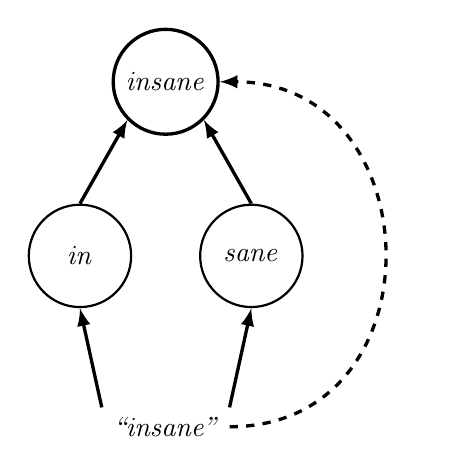
\begin{tikzpicture}[
roundnode/.style={circle, draw=black, very thick, minimum size=1.3cm},
roundnode2/.style={circle, draw=black, thick, minimum size=1.3cm},
roundnode3/.style={rectangle}]

\node[roundnode3]   (main)                                  {};
\node[roundnode2]   (leftcircle)    [left=3mm of main]      {\textit{in}};
\node[roundnode]    (uppercircle)   [above=14mm of main]    {\textit{insane}};
\node[roundnode2]   (rightcircle)   [right=3mm of main]     {\textit{sane}};
\node[roundnode3]   (lowercircle)   [below=18mm of main]    {\textit{``insane''}};

\draw[-latex,very thick] (leftcircle.north) -- (uppercircle.south west);
\draw[-latex,very thick] (rightcircle.north) -- (uppercircle.south east);
\draw[-latex,very thick] (lowercircle.north west) -- (leftcircle.south);
\draw[-latex,very thick] (lowercircle.north east) -- (rightcircle.south);
\draw[-latex,very thick,dashed] (lowercircle.east) .. controls +(right:27mm) and +(right:27mm) .. (uppercircle.east);
\end{tikzpicture}
\caption{Dual-route model of lexical access (\citealt[1045]{Hay2001}; from \citealt[72]{HaspelmathSims2010})}
\label{fig:LexicalAccess}
\end{figure} 

\citet[73]{HaspelmathSims2010} argue that frequently used words (entries) can be accessed more quickly (have greater memory strength) than words used less frequently, and that this is indicative that in their case the direct route is more likely to be chosen. On the other hand, word forms with easily segmentable affixes seem intuitively more likely to be stored according to their morphological parts, i.e. via the decomposition route, since it is the faster method to gain the necessary information. Of course, there are more factors, with a lot of potential for controversy. Be that as it may, I agree with \citet[74]{HaspelmathSims2010} in that ``[w]hile a moderate word-form lexicon ist not very economical, [\dots] it is the most cognitively realistic'', for such lexicon offers both ways of lexical access.

\citet{Zimmermann2019} convincingly demonstrated that the declarative approach is capable to handle Spanish verbal inflections including its regularities and irregularities. In the present paper, I tried to apply the declarative approach to Slovak verbal inflection by examining the majority of regular Slovak paradigmatic verb forms as well as by formulating full word entries and correspondences. I believe to have shown that it is a plausible claim that learners of Slovak make similar generalization. 

\largerpage[1] % avoids widow line on page xxi

As an additional remark, I would like to note that my lexical entries differ from Zimmermann's in that they do not require special features relating to conjugations or thematic vowels. On the other hand, I did not tackle irregular verb forms. Future research will have to fill this gap and should also show how periphrastic structures need to be represented.

\section*{Abbreviations}
\begin{tabularx}{.47\textwidth}{lQ}
\textsc{1/2/3} & first/second/third person \\
\textsc{act} & active voice \\
\textsc{f} & feminine \\
\textsc{ger} & gerund \\
\textsc{imp} & imperative \\
\textsc{ipfv} & imperfective aspect \\
\textsc{inf} & infinitive \\
\textsc{l.ptcp} & \textit{l}-participle \\
\end{tabularx}
\begin{tabularx}{.44\textwidth}{lQ}
\textsc{npst} & non-past\\
\textsc{pass} & passive voice \\
\textsc{pfv} & perfective aspect \\
\textsc{pl} & plural \\
\textsc{pst} & past tense \\
\textsc{ptcp} & participle \\
\textsc{sg} & singular \\
& \\
\end{tabularx}

\section*{Acknowledgements}

I wish to express my gratitude to the editors for inviting me to contribute to the present volume and thus honor Ilse Zimmermann. I learnt a lot from her and keep her in my memory as a truly inspiring linguist. I am also grateful to Berit Gehrke, Uwe Junghanns, and Radek Šimík for many valuable suggestions and corrections.

\sloppy
\printbibliography[heading=subbibliography,notkeyword=this]

% SCHLAGWORTE

\is{Cognition} %add "Cognition" to subject index for this page => add whereever necessary on page
\il{Latin} %add "Latin" to language index for this page => add below example

\end{document}
